
In this chapter, a description of the proposed method is provided. Figure~\ref{fig:architecture} illustrates the overall framework of our approach for text localization, which uses MobileNetV2 as feature extractor and then SSD as multiple text bonding boxes detector. We detail the CNN architectures used, and then explain the learning mechanism used for finding a proper CNN model to the problem. Finally, we present and discuss performed experiments aiming to validate the proposed approach.

\begin{figure}[!ht]
	\centering
	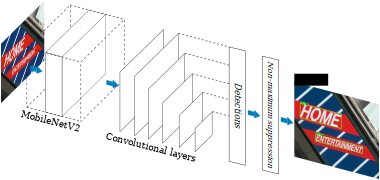
\includegraphics[width=\columnwidth]{ICIP_frankenstein/figs/proposed-method-overview.pdf}
	\caption{Overview of the Proposed Method for Text Localization.}
	\label{fig:architecture}
\end{figure}

\section{Characterization of Text Regions with MobilenetV2}

The MobilenetV2 is a new CNN specifically designed for restricted computing environments that includes two main mechanisms for decreasing the memory footprints and number of operations while keeping the effectiveness of its precursor architecture, the Mobilenet~\cite{Sandler2018CVPR}. Such mechanisms are the linear bottlenecks and the inverted residuals. Besides the depthwise separable convolution operations, which significantly reduce the FLOPS of a neural network, this new version of Mobilenet presents the linear bottleneck mechanism to reduce the number of parameters and keep the accuracy of the network by capturing a low-dimensional subspace (embedded in a manifold formed by a set of activation tensors). The authors claim that non-linearity reduces the capacity of bottleneck features to capture the most representative information. Thus, they decided to use a linear bottleneck, removing the ReLU activation.

The principles that guided the design of the inverted residual layers implemented on MobilenetV2 is that feature maps of the network are able to be encoded in low-dimensional subspaces, and non-linear activation causes some loss of information, notwithstanding their capability to increase representational complexity~\cite{Sandler2018CVPR}.

\begin{figure}[!ht]
	\centering
	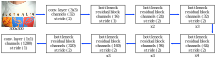
\includegraphics[width=\columnwidth]{ICIP_frankenstein/figs/feature-extraction-v1.pdf}
	\caption{MobilenetV2 architecture used in this work and its parameters. More details on the bottleneck residual block can be found in~\cite{Sandler2018CVPR}.}
	\label{fig:feature-extraction}
\end{figure}

Fig.~\ref{fig:feature-extraction} shows the MobilenetV2 architecture used to characterize text candidate regions. The \textit{bottleneck residual block} implements the optimization mechanisms aforementioned considering the convolutional operations with a kernel of size $3 \times 3$. The first bottleneck block uses an expansion factor of $1$, while the remaining blocks use an expansion factor of $6$, as suggested by \etal{Sandler}~\cite{Sandler2018CVPR}.

\section{Detecting Multiple Instances of Text via SSD}

The localization of text regions in scene images is challenging due to inherent variability of texts, such as size, color, font style, and distortions. 
The text localization should handle multiple scales and bounding boxes with varying aspect ratios. Although several authors consider the image pyramid for performing multi-scale detection, it is quite costly, which may be impractical for a restrictive computing scenario. Thus, we use the Single Shot detector~(SSD) framework~\cite{Liu2016ECCV}, a state-of-the-art method for object detection. The SSD approach includes a multiscale mechanism that allows the identification of text regions in multiple scales on a single inference. Specifically, in the framework, the authors adopt a top-down fusion strategy to build new features with strong semantics while keeping fine details. Text detections are performed based on multiple new constructed features respectively during a single forward pass. All detection results from each layer are refined by means of a non-maximum suppression (NMS) process~\cite{Neubeck2006ICPR}.

\section{Learning}

The main decisions we took in the learning phase of our network are:

\begin{itemize}

\item  {\bf Objective function:}
Similar to \etal{Liu}~\cite{Liu2016ECCV}, we use a multi-task loss function to learn the bounding boxes locations and text/non-text predictions (Equation~\ref{eq:loss}). Specifically, $x_{ij}$ indicates a match ($x_{ij} = 1$) or non-match ($x_{ij} = 0$) between $i$-th default bounding boxes, $j$-th ground-truth bounding boxes, $N$ is the number of matches, $c$ is the ground truth class of the $x_{ij}$ box and the $\alpha$ parameter is used as a multiplier of $\mathcal{L}_{loc}$ to weight the localization loss ($\mathcal{L}_{loc}$) and the confidence loss ($\mathcal{L}_{conf}$). The used loss function can be defined as:
%
\begin{equation}
    L(x,c,l,g) = \frac{1}{N} (\mathcal{L}_{conf}(x,c) + \alpha \mathcal{L}_{loc}(x, l, g))
    \label{eq:loss}
\end{equation}

We adopted the smooth L1 function for $\mathcal{L}_{loc}$ between the predicted box ($l$) and the ground truth box ($g$), and a sigmoid function for $\mathcal{L}_{conf}$. In addition, we set $\alpha=1$ in order to have the localization and confidence components with equal importance.

%\paragraph*{Hard example mining:}
\item {\bf Hard example mining:}
The hard example miner is a mechanism used to prevent imbalances between negative and positive examples during the training phase. On the search for text during the training, we usually have several non-text bounding boxes and few text bounding boxes. To mitigate the training with imbalanced data, we sort the negative bounding boxes according to their confidence, selecting the negative samples with higher confidence value, considering a ratio proportion of 3:1 with the positive samples.

\end{itemize}



%\subsubsection{Linear Bottlenecks}
%
%Beside of depthwise separable convolutions operations, this new version of MobilenetV2 presented the linear bottlenecks in the convolutional blocks aiming reducing the number of parameters of a neural network and capturing the low-dimensional subspace under the supposition that such low-dimensional subspace is embedded in manifold formed by a set of activation tensors. Although the authors did not show a mathematical demonstration that corroborate with this hypothesis, empirical evidences that the use of linear layers is important to prevent non-linearity added from  destroying information. Experiments conducted by the authors shows that non-linear bottlenecks, built with rectified linear units, can decrease the performance significantly in comparison with linear bottlenecks. In other words, the non-linearity can reduce the capacity of bottleneck features in capturing the most representative information.
%
%
%\subsubsection{Inverted residuals bottlenecks} 
%
%For mobile applications and other restrictive computing scenarios, the utilization of computational resources such as memory is crucial since high memory consuming is directly related to battery consumption, besides of provide, in some cases, a negative user experience. To understand how the inverted residual bottlenecks can help in using memory efficiently, we firstly need to understand how the memory-efficient inference works. Basically, a standard implementation builds a directed acyclic compute hyper-graph, in which the nodes represent the tensors and edges represent the operations, and computation (edges) should be scheduled in order to minimize the total number of tensors (nodes).
%


%The SSD-MobilenetV2 model, as described in~\cite{Sandler2018CVPR} was used as a text detector candidate model -- illustrated in Figure~\ref{fig:ssdmobilenet}. The SSDLite is a  mobile-friendly variant of the regular SSD, where the regular convolution layers are replaced by separable convolutions in SSD prediction layers. SSDLite dramatically reduces both parameter count (from 14.8M parameters to 2.1M) and computational cost (1.25B MAdds to 0.25B MAdds) compared to standard SSD. In this model, a Mobilenet V2 is used as a feature extractor for the SSDLite. 
%The MobilenetV2 is a neural network architecture that is designed for mobile and resource-constrained environments, retaining the accuracy of the much bigger and costly models.

